% Written by Luis Perez on August 11, 2014
\documentclass[12pt]{article}
\usepackage{xcolor}
\usepackage{graphicx}
\usepackage{hyperref}
\hypersetup{colorlinks=true, linkcolor=blue, citecolor=blue, filecolor=blue, urlcolor=blue, pdftitle=}

% Set up the margins
\usepackage[margin=1in]{geometry}

% Using packages to display R Code
\usepackage{listings}

% Setting up the title
\title{Testing RDataTracker}
\author{
        Barbara Lerner \\
                Department of Computer Science\\
        Mount Holyoke College\\
        50 College St, South Hadley, MA
            \and
        Emery Boose\\
        Harvard Forest\\
        Harvard University\\
        322 North Main Street, Petersham, MA 
        	\and 
        Luis Antonio Perez \\
        Harvard College \\
        Harvard University \\
        86 Brattle Street, Cambridge, MA
}
\date{\today}

% Pagestyle
\setlength{\headheight}{15pt}
\usepackage{fancyhdr}
\pagestyle{fancy}

% Page header
\fancyhead[R]{Testing RDataTracker}

% Page footer
\pagenumbering{arabic}

% R Code
\lstset{
language=R,
basicstyle=\scriptsize\ttfamily,
commentstyle=\ttfamily\color{gray},
numbers=left,
numberstyle=\ttfamily\color{gray},
stepnumber=1,
numbersep=5pt,
backgroundcolor=\color{white},
showspaces=false,
showstringspaces=false,
showtabs=false,
frame=single,
tabsize=2,
captionpos=b,
breaklines=true,
breakatwhitespace=false,
title=\lstname,
escapeinside={},
keywordstyle={},
morekeywords={},
mathescape
}

\begin{document}

\maketitle

\newpage
\tableofcontents
\listoffigures
\newpage

\section{Regression Testing RDataTracker}

For more information on the RDataTracker Package, look in the ``Using RDataTracker'' document.

\bigskip

Developing new features or fixing bugs on RDataTracker is a long process prone to error; in an attempt to mitigate the number of new bugs introduced with each release, a system for automatically testing RDataTracker has been developed. This system takes advantage of \href{http://ant.apache.org/}{Apache Ant} to automate a series of tests. Each tests consists of two main components: (1) an R script to be tested and (2) a set of expected output files. Ant automates the execution of the script, as well as the comparisons between the output of the script with the expected output files. With this system in place, testing a specific version of a library becomes easy.

\section{Installation}
In order to access the automatic testing system, the following steps need to be taken:
\begin{enumerate}
\item The latest version of the RDataTracker source code must be downloaded. The code is open source and available on \href{https://github.com/blernermhc/RDataTracker}{GitHub}. In particular, make sure you have access to \textbf{build.xml} and \textbf{test.xml}.
\item Install the Java Developer Kit 7. This is a requirement for installing Apache Ant. JDK 7 can be found \href{http://www.oracle.com/technetwork/java/javase/downloads/jdk7-downloads-1880260.html}{here}.
\item Install the latest version of Apache Ant, or at least a version greater that 1.9.1. A working version can usually be found \href{http://ant.apache.org/bindownload.cgi}{here}.
\item If on Windows, it is suggested that you add the Ant bin directory to the PATH variable. Instructions on how to do so can be found \href{http://www.computerhope.com/issues/ch000549.htm}{here}. Otherwise, the commands in the rest of the documentation will need to be modified to account for the fact that the \textbf{ant} command is not directly available at the command prompt.
\end{enumerate}
After the above steps, everything should be set-up to begin using the testing suite. Note that any R dependencies needed by the library will be automatically taken care of by the testing system. More information can be found in Section \ref{sec:add_tests}.

\section{Using the Testing System}
Once the system has been set-up, the process of testing is relatively simple. In this section, we begin with small test cases and move on to the larger automatic test groups. However, it is likely only the largest automatic test groups will ever be executed as they are supersets of the smaller tests. 

\bigskip

In order to simplify the commands outlined later on, we will assume that the terminal/command prompt is currently executing commands inside the main code directory.

\bigskip

If already familiar with \textbf{Apache Ant}, note that the following command will list all the main targets within the system, each with a description.
\begin{lstlisting}
ant -file test.xml -p
\end{lstlisting}
You should see something like Figure \ref{fig:main_test_targets}. Each of these commands is discussed in further detail in this section.

\begin{figure}[!ht]
\caption{Main Test Targets}
\label{fig:main_test_targets}
\begin{center}
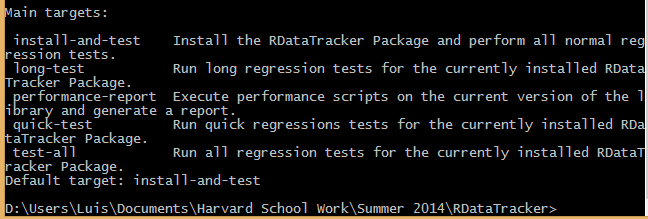
\includegraphics[scale=0.6]{UsingRDataTrackerTests-img/main-out.PNG}
\end{center}
\end{figure}


For a more detailed list of all possible targets, execute:
\begin{lstlisting}
ant -file test.xml -p -verbose
\end{lstlisting}
This will list all possible targets; however, only main targets contain a description. The other targets are useful for Section \ref{section:single_test}.

\subsection{Updating Local Installation of RDataTracker}
Note that most test cases are written so that the version of the RDataTracker Library used is the library currently installed. Therefore, installing the latest version of RDataTracker before runnings tests is imperative. Note that some of the larger test collections perform an automatic installation of the latest source code before executing the tests. 

\bigskip

However, to  manually install the version of the library currently specified by the source code, the following command can be executed:
\begin{lstlisting}
ant install
\end{lstlisting}
The command will run through a series of package checks, then build the package, and then execute a more extensive sequence of package consistency checks, finally installing the library to the default R installation on the local computer. This then allows for the command \textbf{lbrary(RDataTracker)} to load the latest version of the library as opposed to something older. 

\bigskip

The final output from a correct execution of the \textit{install} command should look similar to Figure \ref{fig:success_install}:

\begin{figure}
\caption{Successfull RDataTracker Installation}
\label{fig:success_install}
\begin{center}
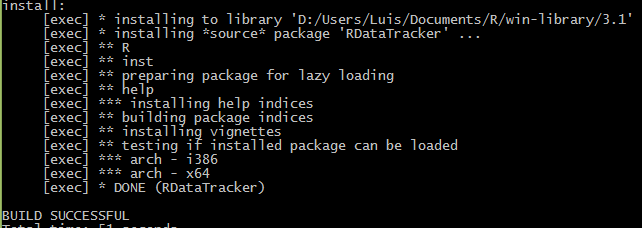
\includegraphics[scale=0.6]{UsingRDataTrackerTests-img/install-out.PNG}
\end{center}
\end{figure}


\subsection{Single Tests}
\label{section:single_test}
The automatic regression testing system makes it possible to execute one single test at a time. In Ant, each test is created from code like the following in conjunction with the \textbf{run-test} target. Note that \textbf{run-test} is not a test itself, but instead code that is reused by other test targets. 
\begin{lstlisting}
<target name="eval-source-test">
 <antcall target="run-test">
   <param name="dir" value="examples/EvalTest"/>
   <param name="out" value="examples/EvalTest/EvalTest-Source.out"/>
   <param name="script-file" value="EvalTest-Source.R"/>
   <param name="expected_out" value="examples/EvalTest/expected_evalTest-Source.out"/>
   <param name="expected_ddg" value="examples/EvalTest/expected_evalTest-Source_ddg.txt"/>
   <param name="source_test" value="true" />
 </antcall>
</target>
\end{lstlisting}

The code above is explained in further detail in Section \ref{sec:add_tests}. However, all that needs to be noted here is the \textbf{target} \textit{name}, from now on referred to as NAME. With NAME known, this single test can be executed using the command:

\begin{lstlisting}
ant -file test.xml NAME
\end{lstlisting}
This simple command executes Ant with NAME as the target from the file \textbf{test.xml}. If the \textbf{-file} flag is not specified, the \textbf{ant} command assumes a file by the name \textbf{build.xml}. While this file is included in repository, its contains code specific to building the RDataTracker package and therefore omission of the \textbf{-file} flag is likely to result in an error. On a successful execution of a test, output like Figure \ref{fig:single_test_out} is to be expected:

\begin{figure}[!ht]
\caption{Output from Single Test}
\label{fig:single_test_out}
\begin{center}
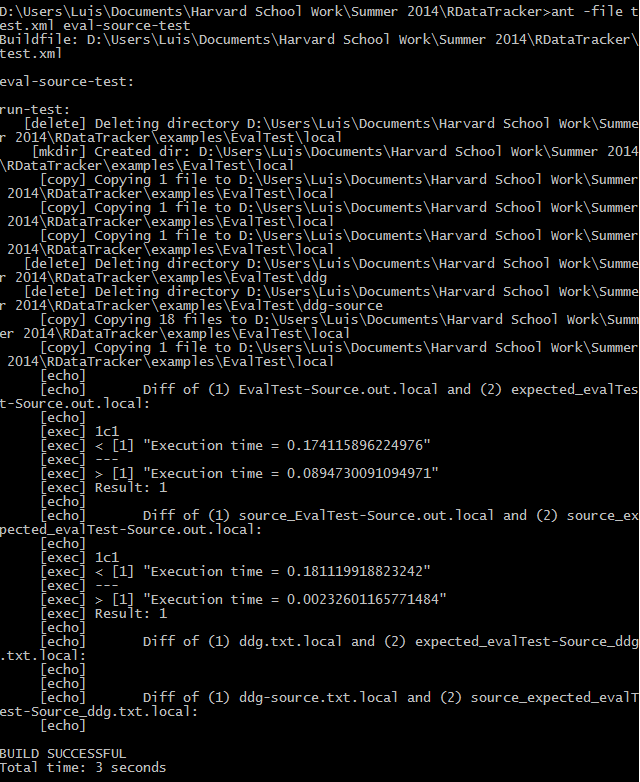
\includegraphics[scale=0.4]{UsingRDataTrackerTests-img/single-test-out.PNG}
\end{center}
\end{figure}
For more information on the meaning of the results above, see Section \ref{section:evaluate_results}.

\bigskip

Note that running a single test only runs the test itself, without ever building, packaging, and installing the latest version of the library. Because all tests use the \textbf{library(RDataTracker)} to load the RDataTracker package, not installing the latest version of the library leads to not \textit{testing} the latest version of the library. 

\subsection{Group Tests}
In order to simplify the testing process, groups of tests have been created to allow multiple, related tests to be executed with single commands. All such groups are created using code like the below inside of \textbf{test.xml}:

\begin{lstlisting}
<target name="console-tests" depends="console-test-1, console-test-2, MismatchedStartFinishBug-test, null-na-test, consoleEdgeCases-test, scope-test, return-test, eval-test, eval-source-test, eval2-test">
	<echo>These automated tests are limited when in console mode. You can always manually check the ouput using diff and the provided expected output files for each script. Do note, however, that all of the tests have also been evaluated using ddg.source, which does in fact capture console commands.</echo>
</target>
\end{lstlisting}

The above code has two main components: (1) the target name and (2) the dependent tests. Additionally, all groups print to stdout an informative message encapsulated by ``$<$echo$> \cdots <$/echo $>$'' The target name, NAME, means that the group tests can be executed with a command just like that in Section \ref{section:single_test}. The tests which are executed are simply those listed under the \textbf{depends} attribute. 

\bigskip

As of the time of writing, the testing library is divided into a few main groups:
\begin{enumerate}
\item \textbf{console-tests} : tests which in some fashion or another heavily depend on the ability to automatically annotate scripts or which work under the assumption of running in an interactive console session. Most of these tests, when run, will normally produce non-informative results, except for when executed using the \textbf{source-test} attribute set as TRUE. For more information on doing this, see Section \ref{section:source_tests}.
\item \textbf{source-tests} : tests which are dedicated to testing the important functionality of \textit{ddg.source}. For more information, see Section \ref{sec:add_tests}.
\item \textbf{script-tests} : test derived from real-world R scripts.
\item \textbf{bug-tests} : tests created to test specific bugs previously encountered with the library and later fixed.
\item \textbf{long-script-tests} : long tests derived from real-world scripts.
\item \textbf{untested-tests} : tests which are not included in \textbf{ANY} other group, usually because their output is not well suited for deterministic comparison.
\end{enumerate}

\subsection{Main Tests}
The main and most useful targets for testing are now explained. The testing system contains a few main sets of tests which serve the purpose of balancing development constraints with correctness of the RDataTracker Library. All of the following targets automatically install the latest version of RDataTracker from source into the R environment, so use with caution. They include:
\begin{enumerate}
\item \textbf{\textit{quick-test}} : this sequence of tests includes all testing groups which are relatively quick to execute and verify. Currently, it excludes only mostly real-word scripts.
\item \textbf{\textit{long-test}} : this sequence of tests includes all testing groups which take a significant amount of time to either evaluate or verify. Currently, this consists mostly of real-world scripts.
\item \textbf{\textit{test-all}} : as the name implies, this sequences of tests includes all tests \textit{suitable} for testing purposes.
\item \textbf{\textit{install-and-test}} : same as \textbf{\textit{test-all}}, but records all output into the file \textbf{test.log} in the root folder of the repository. However, this file is \textbf{NOT} synchronized with the git repository as it has the *.log file extension.
\end{enumerate} 
Again, all of the above targets can be executed with a command similar to that in Section \ref{section:single_test}.
\subsection{Utilities}
\label{sec:utilities}
In addition to tests in the testing suite, two other tools are included to simplify the measurement of performance of the current version of the RDataTracker Library. 
\begin{enumerate}
\item \textbf{\textit{script-timer}} : this utility executes a set of scripts which have been set up to be timed as part of performance review for the currently installed version of the library.  The code used for this utility is entirely contained in the \textit{utilities} folder, with the command code located inside of \textit{script-timer.r}. For more detail, see Section \ref{section:utilities-detail}.\\\\
Output for this target is recorded inside the file \textbf{script-timer.log}. The output from each version of each timed script is separated by multiple blank lines surrounding a single line of the format: \\\\
Execution Time: TIME\_SEC \\\\
The results are stored in a CSV file which is saved under
\begin{lstlisting}
examples/_timingResults/timingData-YYYY-MM-DDTHH.MM.SS.csv
\end{lstlisting}
where the time of execution is used to fill the template file name above.
 
\item \textbf{\textit{script-timer-debug}} : this utility is exactly the same as the above except for the fact that additional output is captured and written out to \textbf{script-timer.log}. The additional output consists of verbose output for each command executed within each of the timed scripts. This allows for more detailed debugging in the case that one of the scripts used for timing RDataTracker has an error.
\item \textbf{\textit{performance-report}} : this utility is a superset of \textit{script-timer}. In addition to performing the tasks above, it further parses the output .csv file and creates a PDF report which plots variables such as execution time, size of ddg directory, and size of script file against each other. The graphs created are self-explanatory. For usability, and to accommodate a wider range of possible execution times for scripts, the scripts are currently grouped into 5 groups, hereafter referred to as GROUP. 
\begin{itemize}
\item All : all timed scripts
\item Fast : timed scripts with execution time up to and including $20$ seconds
\item Moderate : timed scripts with execution time in the range $(20, 60]$ seconds
\item Slow : timed scripts with execution time greater that $1$ minute.
\item Under One Minute : a combination of Fast and Moderate groups.
\end{itemize}

Note that only non-empty groups are included. 

The output report is stored in

\begin{lstlisting}
_plots/report_timingData-YYYY-MM-DDTHH.MM.SS.pdf
\end{lstlisting}
An example title page and graph of the report can be seen in Figure \ref{fig:report_example}:

\begin{figure}[!ht]
\caption{Report Title Page}
\begin{center}
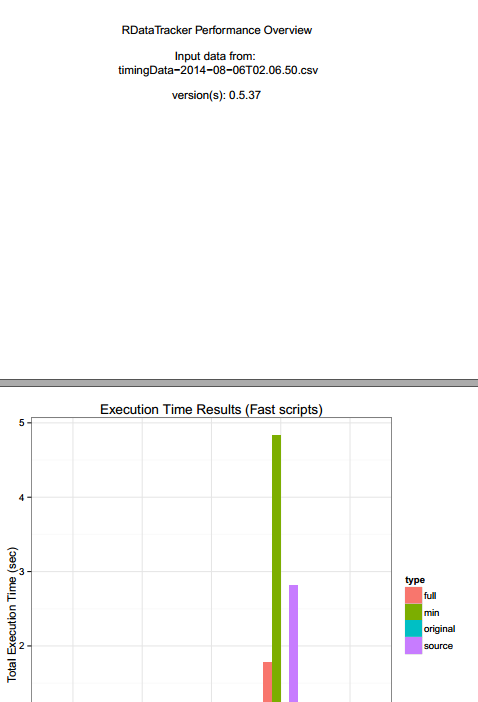
\includegraphics[scale=0.7]{UsingRDataTrackerTests-img/report-example.PNG}
\end{center}
\label{fig:report_example}
\end{figure}

Additionally, subsets of the graphs which are useful to view together are collected, grouped, and saved as pdfs. The reports generated correspond to the non-empty groups above, and are saved under the following naming scheme:
\begin{lstlisting}
_plots/timingData-YYYY-MM-DDTHH.MM.SS/GROUP_timingData-YYYY-MM-DDTHH.MM.SS.pdf
\end{lstlisting} 

Each group is saved into a single PDF (see Figure \ref{fig:group_report}):
\begin{figure}[!ht]
\caption{Group Report}
\begin{center}
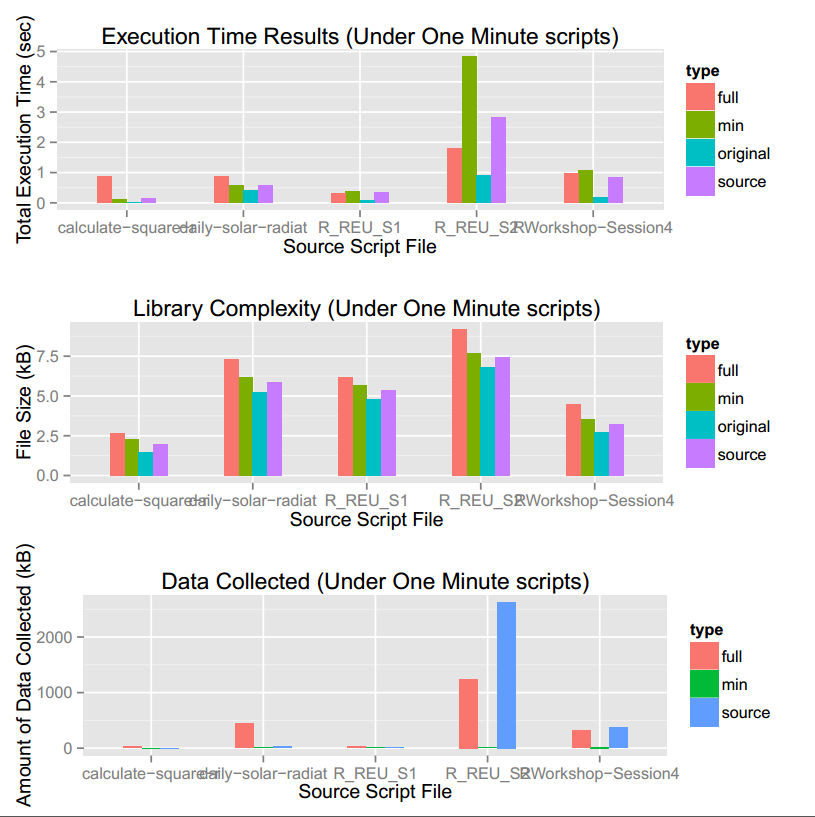
\includegraphics[scale=0.5]{UsingRDataTrackerTests-img/report-group-example.PNG}
\end{center}
\label{fig:group_report}
\end{figure}
\end{enumerate}



\section{Test Details}
\label{section:test_details}
When you run a test, it will create several files named something like:

\begin{enumerate}
\item \textbf{$<$target$>$.out} - standard output from executing the test
\item \textbf{ddg/ddg.txt} - ddg from executing the test
\item \textbf{source\_$<$target$>$.ou}t - standarad output from executing the test with ddg.source
\item \textbf{ddg-source/ddg.txt} - ddg from executing the test with ddg.source
\end{enumerate}

The first 2 output files are running the R script in a batch environment.

The ddg.source results are similar, but not identical to what you would get running in RStudio, selecting all and clicking Run.  Not all tests produce ddg.source outputs.

After the tests are run, the .out files and the ddg.txt files are comparedto expected\_ and source\_expected files with the same names. This comparison is not direct; first, the files are copied to the \textbf{local} directory under the example test. Then, any information which changes with each execution (such as time, as well as relative directories) is removed. For more information, see Section \ref{section:test_details}.

Any other  differences are displayed on standard output.  If the tests work as before, the only  differences you should see are in the execution time. More information on evaluation test results is found in Section \ref{section:evaluate_results}.

Some tests (such as the calculate square roots tests) use random numbers and so produce differences on each execution.  

Additionally, some tests, particularly those that create plots, may produce different 
.out files depending on whether they are run on Mac or PC.

Since the source output is not exactly the same as what you get when running in 
RStudio, it is good to manually test in RStudio at least occasionally.  Two longer
tests that have saved expected results are in the Aaron directory.  There will be
differences due to timestamps so a careful comparison is not possible, but you can at 
least see that there are not large chunks missing or added and that it runs
to completion.  Also, load the ddgs into DDG Explorer and check the error log
at the bottom of the window to make sure there were no problems load the file.  
  
Run in RStudio by loading the file, selecting all and clicking Run:
- Aaron/aaron-min-test.r - compare the ddg written to ddg-min/ddg.txt 
  with expected\_minimal\_console\_ddg.tst
- Aaron/aaron-annotated-test.r - compare the ddg written to ddg-min/ddg.txt 
  with expected\_annotated\_console\_ddg.tst

\subsection{Evaluating Test Results}
\label{section:evaluate_results}
The output of tests results is broken into two major categories:
\begin{itemize}
\item Difference in the .out files
\item Differences in the ddg.txt files
\end{itemize}
These are the first two results shown in the console and recorded by the test results as seen in \ref{fig:single_test_out}. 

Additionally, if the test is run using ddg.source by setting the source parameter to true for the specific test target, then the above results are repeated. Normally, neither of the above should show differences. The only difference should be the execution time.

If the tests stop with Build failed, see what the last test was that was attempted.
Look in its .out file(s).  Most likely, there is something that caused it to 
not work.  Perhaps a library function has changed and the test needs to be
updated.  Perhaps the test needs a network connection and you are not online.
It is usually easy to understand the problem by looking at the .out files.

If a test displays differences and the expected value is the correct value, it 
means that you have introduced a bug into the RDataTracker library.  Figure out
what it is and fix it.

If a test displays differences and the new version is the correct value, you need
to update the expected files. 

\subsection{Updating Test Results}
\label{sec:update_tests}
To update the test results after an update to the library which leads to new expected outputs, you can do the following:

Determine which files to update based on the test output.  Then copy the new result to the expected result file.  Then, edit the expected result, replacing all occurrences of the value used for WorkingDirectory with [DIR].  This enables the comparison functions to ignore changes in the working directory when comparing results with expected, making the tests nicely portable from
one computer to another.  For example, if ddg.txt has:

\begin{lstlisting}
WorkingDirectory="/Users/blerner/Documents/Process/DataProvenance/github/RDataTracker/examples/consoleSource"
\end{lstlisting}  

replace all occurrences of 

\begin{lstlisting}
/Users/blerner/Documents/Process/DataProvenance/github/RDataTracker/examples/consoleSource
\end{lstlisting}

with 

\begin{lstlisting}
[DIR]
\end{lstlisting}


Then, the WorkingDirectory line should read:

\begin{lstlisting}
WorkingDirectory="[DIR]" 
\end{lstlisting}

\textbf{ALL USES OF THE STRING SHOULD BE REPLACED WITH [DIR]} both in the expected 
ddg.txt file and the expected .out file.


\subsection{Adding New Tests}
\label{sec:add_tests}

Adding a new test case to the suite is a relatively simple process. 
\begin{enumerate}
\item Though not necessary, it is preferred to create a new directory under \textbf{examples/} directory. Under this directory, save the R Script containing the code that needs to be tested.
\item Create a new target in the \textbf{test.xml} file. The target follows the format of the other tests, with each parameter now explained. All paths are relative to the root repository directory.
\begin{itemize}
\item \textbf{dir} is the relative directory which encapsulates all files related to the test
\item \textbf{out} is the relative path where the output of the testing script will be saved
\item \textbf{script} is the relative path to the R script containing the code to be tested
\item \textbf{expected\_out} is the relative path to the expected output of the test 
\item \textbf{expected\_ddg} is the relative path to the expected ddg.txt file for the test
\item \textbf{source\_test} is a boolean indicating whether the test script should also be sourced, and the respective output files compared. For information on this, see Section \ref{section:source_tests}.
\end{itemize}
\item If the test depends on additional libraries not normally included with the R installation, then take a look in the file examples/depends.r and modify the section 
\begin{lstlisting}
# List of packages that are needed 
pkgs <- c("RDataTracker", "chron", "gWidgets", "dplR", "zoo", "ggplot2",
		"gdata", "grid", "gridExtra", "mgcv", "akima", "spatstat", "reshape2", "RCurl", "plyr",
    "xkcd", "sysfonts", "extrafont")
\end{lstlisting}
to include the name of the package that is required by your test case. If this is required, the you will also need to modify the target to include a dependency on the target \textbf{dependencies}. Change
\begin{lstlisting}
<target name="TARGET">
...
</target>
\end{lstlisting}
to
\begin{lstlisting}
<target name="TARGET" depends="dependencies">
...
</target>
\end{lstlisting}
\item Execute the target using the testing system and the command for a single test case specified in Section \ref{section:single_test}. This will create the .out files as well as ddg/ddg.txt and ddg-source/ddg.txt (optional).
\item Verify that the DDGs as well as the output files are correct.
\item  With these files created, simple follow the steps in Section \ref{sec:update_tests} to update the test with the correct expected output files.
\end{enumerate}

\subsubsection{Sourcing Tests}
\label{section:source_tests}
A major feature of RDataTracker is the ability to automatically created DDGs from current scripts. This feature relies on what is known as \textbf{ddg.source}. For this reason, the testing suite is capable of testing scripts by sourcing them with ddg.source. The code for this lies inside of the examples/sourceTest.r file, which is copied to the local directory of each test, with the tokens replaced, each time a source test is executed.\\

The steps to update source tests are the same as those outlined in Section \ref{sec:update_tests}. The only difference is the file names. 

\bigskip

When a test script is set up to execute using ddg.source, it contains additional expected output files as well as ddg.txt files which \textbf{must} be named in the exact same way as the normal expected files but with the prefix of ``\textbf{source\_}'' (without the quotes). For example, for a non-source test we might have the files 
\begin{lstlisting}
expected_TEST.out
expected_TEST_ddg.txt
\end{lstlisting}
If the test is modified to be run with \textbf{ddg.source}, we will also need the files
\begin{lstlisting}
source_expected_TEST.out
source_expected_TEST_ddg.txt
\end{lstlisting}
Then, we simply need to modify the target for the test so that the "source\_test" parameter is true.
\begin{lstlisting}
<param name="source_test" value="true" />
\end{lstlisting}

\subsection{Adding Scripts to Utilities}
\label{section:utilities-detail}
In addition to testing, as described in Section \ref{sec:utilities}, the testing suite is also capable of collecting data and generating a report on the performance of the current version of RDataTracker. However, this feature was added on later to the testing suite, and therefore, does not automatically test all current tests. Instead, one must add a test.

\bigskip
To add a test to the performance review section of the testing suite, only two files need to be created. It is recommended that these two files are created inside the folder of a current test script, or a new folder be created to hold the results.
\begin{enumerate}
\item A file with the pattern SCRIPTNAME-clean.r which contains a completely clean, unmodified version of the script to be timed.
\item A file with the pattern template\_SCRIPTNAME-annotated.r which contains a fully instrumented version of the script to be timed. However, this script should contain no information about the initialization of the DDG or the saving of the DDG. All of this is added automatically later.
\item Add any dependent libraries to examples/depends.r as instructed in Section \ref{sec:add_tests}.
\end{enumerate}

Once the two files above have been added, the target mentioned in Section \ref{sec:utilities} can be executed and successfully run. The added file will be automatically included in the results.

\subsubsection{More Details}
The timing system relies on the two files mentioned in Section \ref{section:utilities-detail}. It only requires two files because the minimal instrumentations are done automatically. The files which are executed and timed can be found in the localTimingScripts directory created within the folder containing the two aforementioned files.

NOTE: The system looks for files with the ``-clean'' suffix to find scripts which need to be timed. If no file with the ``template\_'' prefix and ``-annotated''  suffix is found, then the results for the ``Annotated'' version of the script will be incorrect as a clean version of the script is executed instead. 

\newpage

\section{Future Work}
\begin{itemize}
\item Tie the correctness and performance functionalities of the testing system together. It should be the case that scripts are only timed after they have been checked for correctness.
\item Additionally, it should be possible to time all current tests cases.
\item Modify the graph group PDFs (see Figure \ref{fig:group_report}) so that the formatting is always correct, no matter the number of scripts or the length of the script names.
\end{itemize}

\end{document}
